\documentclass{article}
\usepackage{graphicx}
\usepackage[margin=1.5cm]{geometry}
\usepackage{amsmath}

\begin{document}

\title{Tuesday Reading Assessment: Unit 7, Power and Conservation of Energy}
\author{Prof. Jordan C. Hanson}

\maketitle

\section{Memory Bank}

\begin{enumerate}
\item $KE = \frac{1}{2}m v^2$ ... Definition of kinetic energy
\item $P = \Delta E / \Delta t$ ... Definition of power
\item 1 calorie is 4.184 Joules
\item 1 kcal is 4184 Joules
\end{enumerate}

\begin{figure}[ht]
\centering
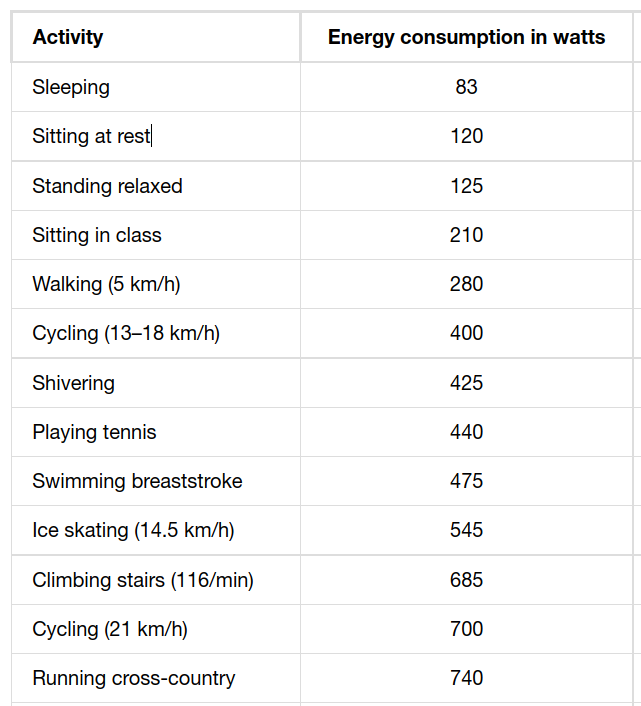
\includegraphics[width=0.4\textwidth]{powertable.png}
\caption{\label{fig:powertable}}
\end{figure}

\section{Work, Power, and the Human Body}

\begin{enumerate}
\item Suppose you are attending a conference for four hours, where you will be mostly be sitting and concentrating on speakers and workshops. (a) How many Watts does this require?  (b) If the conference is four hours long, how many Joules in total do you expect to burn? (c) How many kcal is this?  Is it much larger than or smaller than 2,000? \\ \vspace{1cm}
\item Based on the prior exercise, determine how many kcal would be necessary to run cross-country for four hours.
\end{enumerate}
\end{document}